%%%%%%%%%%%%%%%%%%%%%%%%%%%%%%%%%%%%%%%%%%%%%%%%%%%%%%%%
%                IAML 2020 Assignment 2                %
%                                                      %
%                                                      %
% Authors: Hiroshi Shimodaira and JinHong Lu           %
% Based on: Assignment 1 by Oisin Mac Aodha, and       %
%          Octave Mariotti                             %
% Using template from: Michael P. J. Camilleri and     %
% Traiko Dinev.                                        %
%                                                      %
% Based on the Cleese Assignment Template for Students %
% from http://www.LaTeXTemplates.com.                  %
%                                                      %
% Original Author: Vel (vel@LaTeXTemplates.com)        %
%                                                      %
% License:                                             %
% CC BY-NC-SA 3.0                                      %
% (http://creativecommons.org/licenses/by-nc-sa/3.0/)  %
%                                                      %
%%%%%%%%%%%%%%%%%%%%%%%%%%%%%%%%%%%%%%%%%%%%%%%%%%%%%%%%

%--------------------------------------------------------
%   IMPORTANT: Do not touch anything in this part
\documentclass[12pt]{article}
%%%%%%%%%%%%%%%%%%%%%%%%%%%%%%%%%%%%%%%%%
% Cleese Assignment
% Structure Specification File
% Version 1.0 (27/5/2018)
%
% This template originates from:
% http://www.LaTeXTemplates.com
%
% Author:
% Vel (vel@LaTeXTemplates.com)
%
% License:
% CC BY-NC-SA 3.0 (http://creativecommons.org/licenses/by-nc-sa/3.0/)
% 
%%%%%%%%%%%%%%%%%%%%%%%%%%%%%%%%%%%%%%%%%

%----------------------------------------------------------------------------------------
%	PACKAGES AND OTHER DOCUMENT CONFIGURATIONS
%----------------------------------------------------------------------------------------

\usepackage{lastpage} % Required to determine the last page number for the footer
\usepackage{graphicx} % Required to insert images
\setlength\parindent{0pt} % Removes all indentation from paragraphs
\usepackage[most]{tcolorbox} % Required for boxes that split across pages
\usepackage{booktabs} % Required for better horizontal rules in tables
\usepackage{listings} % Required for insertion of code
\usepackage{etoolbox} % Required for if statements
\usepackage{geometry} % Required for adjusting page dimensions and margins
\usepackage[utf8]{inputenc} % Required for inputting international characters
\usepackage[T1]{fontenc} % Output font encoding for international characters
\usepackage{fancyhdr} % Required for customising headers and footers
\usepackage{xspace}
\usepackage{booktabs}
\usepackage[colorlinks]{hyperref}
\usepackage{etoolbox}

\newcommand{\ie}{i.e.\@\xspace}
\newcommand{\eg}{e.g.\@\xspace}
\newcommand{\notemark}[1]{\textcolor{blue}{N.B.\ \emph{#1}}}
\newcommand{\noteself}[1]{\textcolor{red}{Thought: \emph{#1}}}
\newcommand{\note}[1]{\emph{\textbf{N.B.}\@\xspace#1}}
\newcommand{\hint}[1]{\emph{Hint: #1}}
\newcommand{\half}{$\frac{1}{2}$ }

\newbool{clearnext}		%Running Counter to see if clearing the page or not in the next subquestion.
\newbool{clearon}		%Parameter for specifying whether we will be clearing or not.
\newbool{authoron}		%Parameter to specify whether to show author or not

%----------------------------------------------------------------------------------------
%	Standard Template
%----------------------------------------------------------------------------------------
\geometry{
	paper=a4paper, % Change to letterpaper for US letter
	top=3cm, % Top margin
	bottom=3cm, % Bottom margin
	left=2.5cm, % Left margin
	right=2.5cm, % Right margin
	headheight=14pt, % Header height
	footskip=1.4cm, % Space from the bottom margin to the baseline of the footer
	headsep=1.2cm, % Space from the top margin to the baseline of the header
	%showframe, % Uncomment to show how the type block is set on the page
}
\pagestyle{fancy} % Enable custom headers and footers

%----------------------------------------------------------------------------------------
%	My Changes
%----------------------------------------------------------------------------------------
\lhead{\small\assignmentClass}
\chead{}
\ifbool{authoron}{\rhead{\small{\assignmentAuthorName}}}{\rhead{}}

\lfoot{} % Left footer
\cfoot{} % Centre footer
\rfoot{\small Page\ \thepage\ of\ \pageref*{LastPage}} % Right footer

\renewcommand\headrulewidth{0.5pt} % Thickness of the header rule

%----------------------------------------------------------------------------------------
%	MODIFY SECTION STYLES
%----------------------------------------------------------------------------------------

\usepackage{titlesec} % Required for modifying sections

%------------------------------------------------
% Section

\titleformat
{\section} % Section type being modified
[block] % Shape type, can be: hang, block, display, runin, leftmargin, rightmargin, drop, wrap, frame
{\Large\bfseries} % Format of the whole section
{\assignmentQuestionName~\thesection} % Format of the section label
{6pt} % Space between the title and label
{} % Code before the label

\titlespacing{\section}{0pt}{0.5\baselineskip}{0.5\baselineskip} % Spacing around section titles, the order is: left, before and after

%------------------------------------------------
% Subsection

\titleformat
{\subsection} % Section type being modified
[block] % Shape type, can be: hang, block, display, runin, leftmargin, rightmargin, drop, wrap, frame
{} % Format of the whole section
{\bf{\arabic{section}.\arabic{subsection}}} % Format of the section label
{4pt} % Space between the title and label
{} % Code before the label

\titlespacing{\subsection}{0pt}{0.5\baselineskip}{0.5\baselineskip} % Spacing around section titles, the order is: left, before and after

% \renewcommand\thesubsection{(\alph{subsection})}
\renewcommand\thesubsection{\arabic{section}.\arabic{subsection}}

%----------------------------------------------------------------------------------------
%	CUSTOM QUESTION COMMANDS/ENVIRONMENTS
%----------------------------------------------------------------------------------------

% Environment to be used for each question in the assignment
\newenvironment{question}[1]{
	\ifbool{clearon}{\clearpage}{}
	\global\setbool{clearnext}{false}
	\vspace{0.5\baselineskip} % Whitespace before the question
	\section{: #1}
	\lfoot{\small\itshape\assignmentQuestionName~\thesection~continued on next page\ldots} % Set the left footer to state the question continues on the next page, this is reset to nothing if it doesn't (below)
}{
	\lfoot{} % Reset the left footer to nothing if the current question does not continue on the next page
}

%------------------------------------------------

% Environment for inter-subquestion texts (no arguments)
\newenvironment{interquestiontext}{
	\ifbool{clearon}{\ifbool{clearnext}{\clearpage}{}}{}
	\global\setbool{clearnext}{false}
}{
}

%------------------------------------------------


%------------------------------------------------

% Environment for subquestions, takes 1 argument - the name of the section
\newenvironment{subquestion}[1]{
	\ifbool{clearon}{\ifbool{clearnext}{\clearpage}{}}{}
	\global\setbool{clearnext}{true}
	\subsection{#1}
}{
}

%------------------------------------------------

% Command to print a question sentence
\newcommand{\questiontext}[1]{
	\textbf{#1}
	\vspace{0.5\baselineskip} % Whitespace afterwards
	\global\setbool{clearnext}{false}
}

%------------------------------------------------
% Command to print a  Marking Scheme box.
\newcommand{\marking}[1]{
	\begin{tcolorbox}[colback=green!5!white,enhanced]
		\textbf{Marking Scheme:}#1
	\end{tcolorbox}
}

%------------------------------------------------

% Command to print a box that breaks across pages with the space for a student to answer
\newenvironment{model}[1]{
\begin{tcolorbox}[enhanced]
\textbf{Model Answer}:
#1
}
{
\end{tcolorbox}
}

\newenvironment{answerbox}[1]{
\begin{tcolorbox}[enhanced, height=#1]
}
{
\end{tcolorbox}
}



%------------------------------------------------

% Command to print an assignment section title to split an assignment into major parts
\newcommand{\assignmentSection}[1]{
	{
		\centering % Centre the section title
		\vspace{2\baselineskip} % Whitespace before the entire section title
		
		\rule{0.8\textwidth}{0.5pt} % Horizontal rule
		
		\vspace{0.75\baselineskip} % Whitespace before the section title
		{\LARGE \MakeUppercase{#1}} % Section title, forced to be uppercase
		
		\rule{0.8\textwidth}{0.5pt} % Horizontal rule
		
		\vspace{\baselineskip} % Whitespace after the entire section title
	}
}

%----------------------------------------------------------------------------------------
%	TITLE PAGE
%----------------------------------------------------------------------------------------

\title{
	\thispagestyle{empty} 		% Suppress headers and footers
	\vspace{0.01\textheight} 	% Whitespace before the title
        \hfill {\normalsize \it Ver.~1.0.0}\\
	\textbf{\assignmentClass:\\ \assignmentTitle}\\[4pt]
	\ifbool{authoron}{\assignmentAuthorName}{
	\ifdef{\assignmentDueDate}{{\small Due\ on\ \assignmentDueDate}\\}{}
	{\large \textit{\assignmentWarning}}
	\vspace{0.01\textheight}} % Whitespace before the author name
}

\ifbool{authoron}{\author{Student: \textbf{\assignmentAuthorName}}}{}
\date{} % Don't use the default title page date field

% by Hiroshi
\usepackage{bm}
\newcommand{\VEC}[1]{\ensuremath{\bm{#1}}}
\newcommand{\refQ}[1]{Question~\ref{#1}}
\hypersetup{linkcolor=blue}




% Options for Formatting Output

\global\setbool{clearon}{true} %
\global\setbool{authoron}{true} %
\ifbool{authoron}{\rhead{\small{\assignmentAuthorName}}\cfoot{\small{\assignmentAuthorName}}}{\rhead{}}



\newcommand{\assignmentQuestionName}{Question}
\newcommand{\assignmentTitle}{Assignment\ \#2}

\newcommand{\assignmentClass}{IAML -- INFR10069 (LEVEL 10)}

\newcommand{\assignmentWarning}{NO LATE SUBMISSIONS} % 
\newcommand{\assignmentDueDate}{Monday,\ November\ 23,\ 2020 @ 16:00}
%--------------------------------------------------------



%%%%%%%%%%%%%%%%%%%%%%%%%%%%%%%%%%%%%%%%%%%%%%%%%%%%%%%
%
% NOTE: YOU NEED TO ENTER YOUR STUDENT ID BELOW.
%
%%%%%%%%%%%%%%%%%%%%%%%%%%%%%%%%%%%%%%%%%%%%%%%%%%%%%%%% 
% --------------------------------------------------------
% IMPORTANT: Specify your Student ID below. You will need to uncomment the line, else compilation will fail. Make sure to specify your student ID correctly, otherwise we may not be able to identify your work and you will be marked as missing.
\newcommand{\assignmentAuthorName}{s1803764}
%--------------------------------------------------------



\begin{document}


%%%%%%%%%%%%%%%%%%%%%%%%%%%%%%%%%%%%%%%%%%%%%%%%%%%%%%%%%%%%%%%%%%%%%%%%%%%%%%
%============================================================================%
%%%%%%%%%%%%%%%%%%%%%%%%%%%%%%%%%%%%%%%%%%%%%%%%%%%%%%%%%%%%%%%%%%%%%%%%%%%%%%
\clearpage
%
% Question 1
%

\begin{question}{(30 total points) Image data analysis with PCA}

  
  \questiontext{In this question we employ PCA to analyse image data}
  

  
  \medskip

   %==============================
   % Q1.1
  \begin{subquestion}{(3 points)
      Once you have applied the normalisation from Step 1 to Step 4 above,
      report the values of the first 4 elements for the first training
      sample in \texttt{Xtrn\_nm},
      i.e. \texttt{Xtrn\_nm[0,:]} and the last training sample,
      i.e. \texttt{Xtrn\_nm[-1,:]}.
    } \label{Q1.1}
    

      \begin{answerbox}{10em}
        \begin{center}
        \textbf{\underline{First 4 elements of the first and last samples from the}}\\
        \textbf{\underline{normalized training dataset Xtrn\_nm}}
        \vspace{0.3cm}\\
         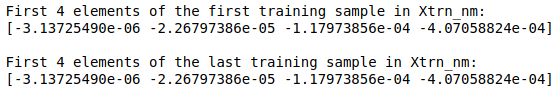
\includegraphics[width=0.9\textwidth]{images/q11.png}
        \end{center}
      \end{answerbox}
  


   \end{subquestion}
   %
   % ==============================
   % 
   % Q1.2
   \begin{subquestion}{(4 points)
      Using {\tt Xtrn} and Euclidean distance
      measure, for each class,
      find the two closest samples and two furthest
      samples of that class to the mean vector of the class.
    }  \label{Q1.2}




  \begin{answerbox}{52em}
    \begin{center}
    \textbf{\underline{A grid to show the mean vectors for each class along with the}}\\
    \textbf{\underline{closest and furthest samples from these means}}
    \vspace{0.2cm}\\
    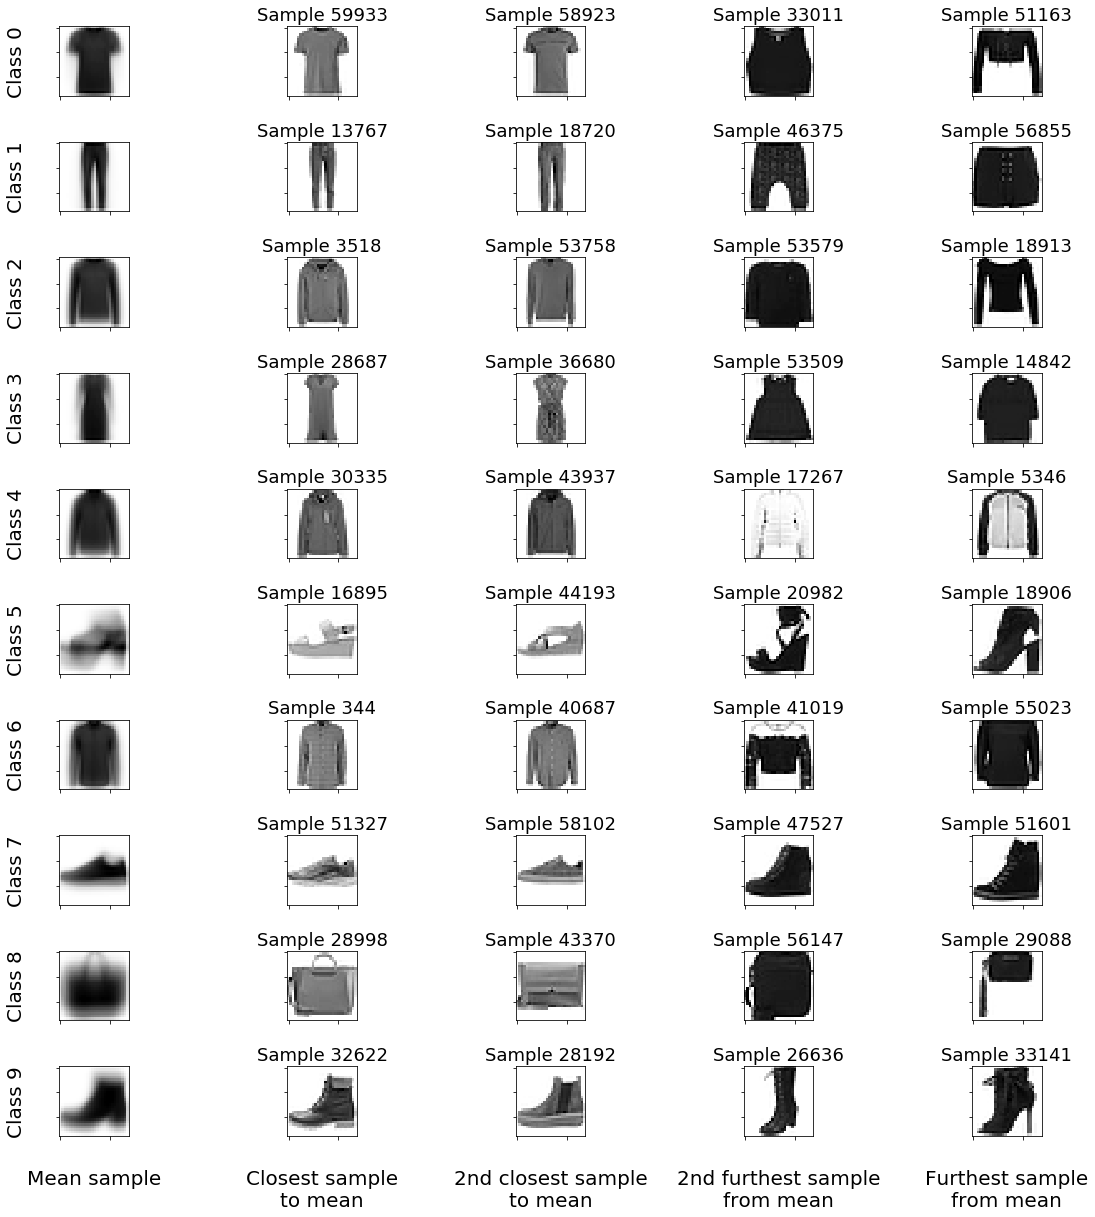
\includegraphics[width=0.8\textwidth]{images/q12.png}
    \end{center}
    \footnotesize{\textbf{\underline{Analysis of our results}}}\\
\\
    \scriptsize{
    There is an interesting trend amongst the closest and furthest samples for each given class in the dataset. Notice that all the 'closest' samples are a subtle gray, and in contrast all the 'furthest' samples are very dark or very light (eg. the class 4 samples). We can deduce that this is due to the fact that the intensely dark/light colour pixels magnify the difference (and thus Euclidean distance) between corresponding pixel values in different samples.\\
\\
    This is a very important observation as it highlights the significance of colour intensity when calculating the similarity between different samples. This colour intensity could ultimately skew the performance of our classifier when predicting the type of clothing for uniquely dark/light samples. This is especially problematic if a given class (type of clothing) is more likely to be dark/light as this will make it more likely to classify uniquely dark/light samples from other classes.\\
\\
    To prevent this issue, given that we are classifying the type of clothing and not the colour, we could either use a method specifically for classifying shapes (image segmentation) or we could normalize the colour intensity of samples upon input (normalize the values of the pixels to be within a certain range).}
  \end{answerbox}



   \end{subquestion}

   % 
   % Q1.3
   \begin{subquestion}{(3 points)
       Apply Principal Component Analysis (PCA) to the data of {\tt
         Xtrn\_nm} using \href{https://scikit-learn.org/0.19/modules/generated/sklearn.decomposition.PCA.html}{sklearn.decomposition.PCA}, and report the variances of projected data for the first five principal components in a table.
        Note that you should use {\tt Xtrn\_nm} instead of {\tt Xtrn}.
     } \label{Q1.pca.variance}



    \begin{answerbox}{15em}
        \begin{center}
        \textbf{\underline{Calculating the variances of the projected data in Xtrn\_nm}}\\
        \textbf{\underline{for the first five principal components}}\\
        \vspace{0.5cm}
        \footnotesize{
        \begin{tabular}{ |c|c| } \hline
        \textbf{Principal Component \#} & \textbf{Explained Variance} \\ \hline
        1 & 19.81 \\
        2 & 12.112 \\
        3 & 4.106 \\
        4 & 3.382 \\
        5 & 2.625 \\\hline
        \end{tabular}
        }
        \end{center}
    \end{answerbox}
    


   \end{subquestion}

   %==============================
   % Q1.4
   \begin{subquestion}{(3 points)
       Plot a graph of the cumulative explained variance ratio as a function of the number of principal components, $K$, where $1\le K \le 784$.
       Discuss the result briefly.
     } \label{Q1.plot.pca.variance}
   

      \begin{answerbox}{30em}
        \begin{center}
         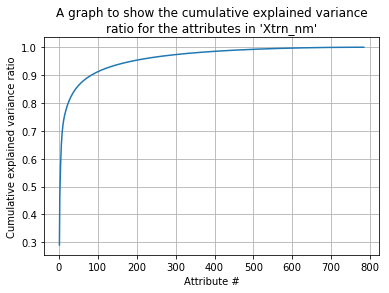
\includegraphics[width=0.6\textwidth]{images/q14.png}
        \end{center}
        \scriptsize{
        \textbf{\footnotesize{\underline{Analysis of our results}}}\\
        This cumulative explained variance ratio ultimately represents how much detail our new data retains from our original data. The reason the 'detail' of our data is measured by variance is because variance measures the average difference between all samples in the data, we want data with a high variance as this allows for more accurate classification. Given this information it is evident to see that this graphing model ultimately represents the relationship between the 'detail' in the data and the number of dimensions. This is very useful when you have high dimensional data that you want to reduce whilst still keeping as much 'detail' in the data as possible.\\
\\
        \textbf{We can see from the figure above that using just 100 dimensions (about 87.24\% less data) already secures about 91.17\% of the total cumulative variance from the original data.}\\
\\
        Choosing the optimal number of dimensions for a given dataset depends entirely on the context of the data/classification model, as this directly denotes how important the trade-off between the size of the data and the quality of the data is. For example, when working with critical data we can not afford to lose any quality thus we would prefer to not reduce the dimensions. However, reducing dimensions can be very useful for many supervised methods, making problems that are not linearly seperable into ones that are, reducing noise in the data, and being able to visually represent high-dimensional data.
        }
      \end{answerbox}
  


   \end{subquestion}

   %==============================
   % Q1.5
   \begin{subquestion}{(4 points)
      Display the images of the first 10 principal components in
      a 2-by-5 grid, putting the image of 1st principal component on
      the top left corner, followed by the one of 2nd component to the right.
      Discuss your findings briefly.
     } \label{Q1.disp.pca}
   

      \begin{answerbox}{35em}
        \begin{center}
        \textbf{\underline{A grid to show the images of the first 10 principal components}}
        \vspace{0.25cm}\\
         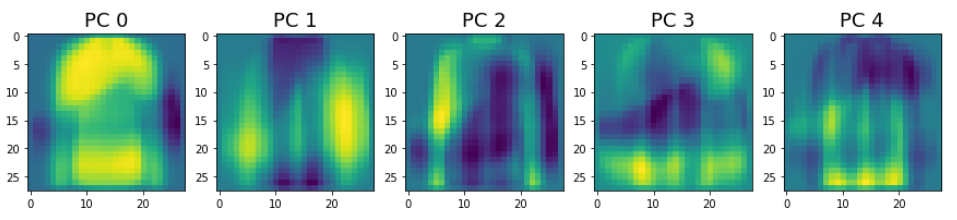
\includegraphics[width=0.73\textwidth]{images/q151.png}
         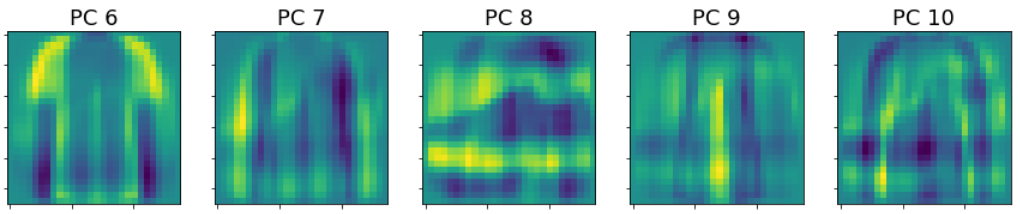
\includegraphics[width=0.73\textwidth]{images/q152.png}
        \end{center}
        \scriptsize{
        \emph{**These images represent the eigenvectors for each of their respective dimensions. Each of these eigenvectors has a direction and a corresponding eigenvalue. These are used for projecting data into new spaces.}\\
\\
        \textbf{\footnotesize{\underline{Analysis of our results}}}\\
\\
        What is useful is that we notice that many of the different clothing shapes are retained in these eigenvectors. In most of these images you can see the resemblances of most of the different clothing types from our dataset, however, what is truly interesting is the frequency and intensity of the different clothing shapes found amongst these. These factors are very important as these suggest what are the most significant features throughout all of our different classes for classification.\\
\\
        With regards to the frequency of the different clothing shapes, I am referring to the number of eigenvectors in which we can visibly see the resemblance of the different clothing types. For example, in contrast to other clothing shapes, we can see in almost all of the images the resemblance of a long sleeved shirt. This ultimately suggests that this long sleeved shirt shape was most common from our training data. We know this is not due to class imbalance in our training dataset as we used an equal number of samples for each class, but rather due to the similarity between different classes. This is evident as illustrated by the class images in Q1.2 where classes 2 (pullover), 4 (coat) and 6 (shirt) all appear to take very similar shapes, resembling that of a long sleeved shirt.\\
\\
        With regards to the intensity of the different clothing shapes, I am referring to the most prominent/visible shapes for each eigenvector. For example, PC 1 shows the resemblance of a long sleeved shirt, PC 2 shows the resemblance of trousers, PC 3 shows the resemblance of a boot, and PC 4 shows the resemblance of a sneaker. This ultimately represents how the seperate dimensions in our dataset may be used predominantly for classifying certain classes. This makes perfect sense as this allows our model to apply different weightings to each dimension.
}
      \end{answerbox}
  


   \end{subquestion}

   %==============================
   % Q1.6
   \begin{subquestion}{(5 points)
       Using \texttt{Xtrn\_nm}, 
       for each class and for each number of principal components $K =
       5, 20, 50, 200$, apply dimensionality reduction with PCA to the
       first sample in the class, reconstruct the sample from the
       dimensionality-reduced sample, and 
       report the Root Mean Square Error (RMSE) between the
       original sample in {\tt Xtrn\_nm} and reconstructed one.
     } \label{Q1.6}

     

      \begin{answerbox}{25em}
        \begin{center}
        \textbf{\underline{A table to show the RMSE between the original and the reconstructed}}\\
        \textbf{\underline{version of the first sample for every class with varying numbers}}\\
        \textbf{\underline{of PCA components (K)}} \\
        \vspace{0.3cm}
        \footnotesize{*Each class sample is reconstructed by reducing the sample to K dimensions and then transforming it back to the original number of dimensions, this is all done via the sklearn PCA implementation.\\
        \vspace{0.5cm}
        \begin{tabular}{ |c|c|c|c|c|c| } \hline
            \textbf{RMSE} & K = 5 & K = 20 & K = 50 & K = 200 \\ \hline
            Class = 0 & 0.256 & 0.15 & 0.128 & 0.063 \\
            Class = 1 & 0.198 & 0.14 & 0.095 & 0.037 \\
            Class = 2 & 0.199 & 0.146 & 0.124 & 0.08 \\
            Class = 3 & 0.146 & 0.107 & 0.083 & 0.056 \\
            Class = 4 & 0.118 & 0.103 & 0.088 & 0.045 \\
            Class = 5 & 0.181 & 0.159 & 0.142 & 0.09 \\
            Class = 6 & 0.129 & 0.096 & 0.072 & 0.045 \\
            Class = 7 & 0.166 & 0.128 & 0.106 & 0.063 \\
            Class = 8 & 0.223 & 0.145 & 0.124 & 0.094 \\
            Class = 9 & 0.184 & 0.151 & 0.122 & 0.072 \\
            \hline
        \end{tabular}
        }
        \end{center}
      \end{answerbox}
  


   \end{subquestion}
   
   %==============================
   % Q1.7
   \begin{subquestion}{(4 points)
       Display the image for each of the reconstructed samples in
       a 10-by-4 grid, where each row corresponds to a class and
       each row column corresponds to a value of $K=5, \; 20, \; 50, \; 200$.
     } \label{Q1.7}


   

      \begin{answerbox}{52em}
        \begin{center}
        \textbf{\underline{A grid to show the images of the reconstructed class samples for}}\\
        \textbf{\underline{varying amounts of dimension reductions (K)}}
        \vspace{0.3cm}\\
         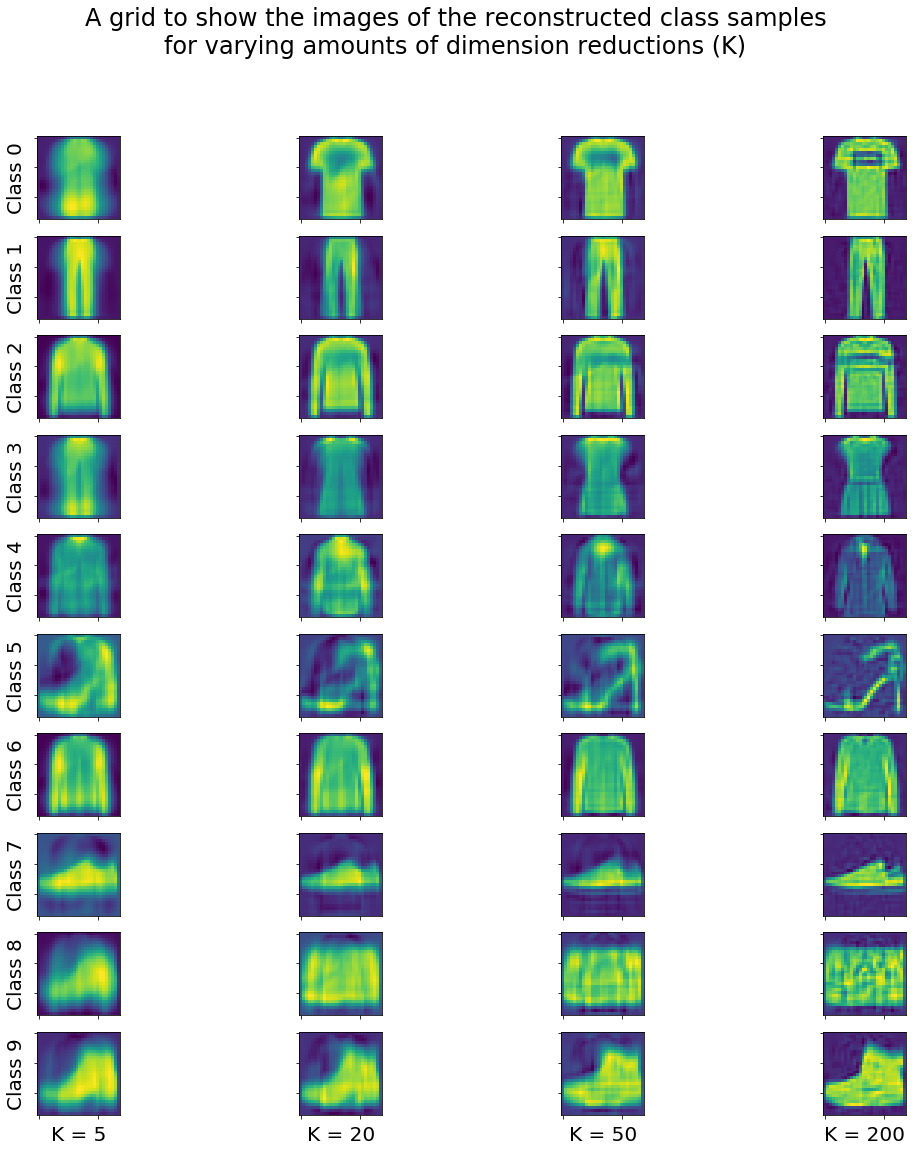
\includegraphics[width=0.84\textwidth]{images/q17.png}
        \end{center}
        \footnotesize{\textbf{\underline{Analysis of our results}}}\\
        \scriptsize{
\\
        As expected the reconstructed samples become more detailed as we increase the value of K. This is evident due to the increased number of dimensions to retain detail within the data.\\
\\
        PCA reduces dataset dimensions by choosing dimensions which maximize the variance in the data, this is evident to see as the reconstructed samples with small K highlight the more promiment features from their respective original samples.\\
\\
        What I found particularly interesting is that for K=5 the reconstructed class 8 sample appears to have taken the shape of a shoe (from a bag), and the reconstructed class 3 sample appears to have taken the shape of a pair of trousers (from a dress). We can imagine the lost detail in our data from PCA ultimately made the reconstruction of 5D samples more similar to different (and thus incorrect) classes. This problem is due to the fact that PCA is unsupervised, a good solution to this would be to instead use a supervised dimensionality reduction method such as LDA.}
      \end{answerbox}
  


   \end{subquestion}
   %==============================
   %
   %==============================
   % Q1.8
   \begin{subquestion}{(4 points)
       Plot all the test samples (\texttt{Xtrn\_nm}) on the
       two-dimensional PCA plane you obtained in \refQ{Q1.pca.variance}, where each sample is
       represented as a small point with a colour specific to the class of
       the sample.  Use the 'coolwarm' colormap for plotting.
     } \label{Q1.8}


   

      \begin{answerbox}{40em}
        \begin{center}
        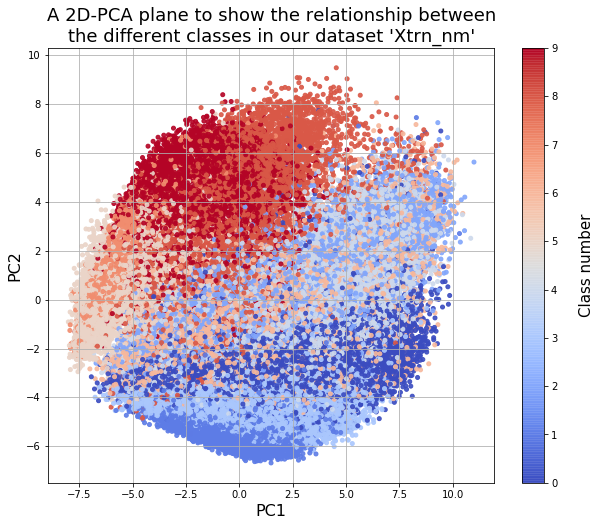
\includegraphics[width=0.6\textwidth]{images/q18.png}
        \end{center}
        \footnotesize{\textbf{\underline{Analysis on the seperations/congregations of class samples}}}\\
        \\
        \scriptsize{
        As expected from our analysis in Q1.5 classes 2 (pullover), 4 (coat) and 6 (shirt) have very similar trends in their data comprising most of the data in the middle of this set of scatter points (almost following a y=x diagonal). This is evidently due to their similarity in shapes, all resembling a long sleeved shirt. We can deduce that these points are in the middle of this scatter due to their frequency of shape (as discussed in Q1.5). Directly below this collection of classes we can see that class 0 (T-shirt) follows a similar trend, this is evidently due to it also being the shape of a shirt but with the slight difference of short sleeves.\\
\\
        We can also see on the left side of the scatter the congregation of the samples from classes 5 (sandals), 7 (sneaker), and 9 (ankle boots). This is evidently due to their similarity in shapes given that they are all different types of shoes. As expected, class 7 (sneaker) makes up the middle of this congregation of points, this is due to the fact that a sneaker is more similar to both a sandal and an ankle boot than they are to each other. At the very top of the scatter is class 8 (bag) which seems to merge into class 9 (ankle boots) quite alot. I found this quite surprising initially but realized this similarity can be attributed to the typical wideness we see in both boots and bags (as shown by the means in Q1.2).\\
\\
        The most consistent/unique of all classes is that of class 1 (trouser) at the very bottom of the scatter. This consistency is evident due to the very pure section of blue. We can deduce this consistency is due to the uniqueness in shape of a pair of trousers. This is evident when we notice the narrowness of a pair of trousers in comparison to other classes (as illustrated by the mean in Q1.2), and the gap between trouser legs which exclude the points in the center of the image which practically all other classes make use of.\\
\\
        Just above class 1 (trouser) and below class 0 (T-shirt) is class 3 (dress). This makes sense due to a dress' short sleeves (like a t-shirt) and narrowness (like a pair of trousers - again illustrated by the mean in Q1.2).
        }
      \end{answerbox}
  


   \end{subquestion}
   %
   %==============================
   

\end{question}
%%%%%%%%%%%%%%%%%%%%%%%%%%%%%%%%%%%%%%%%%%%%%%%%%%%%%%%%%%%%%%%%%%%%%%%%%%%%%%
%============================================================================%
%%%%%%%%%%%%%%%%%%%%%%%%%%%%%%%%%%%%%%%%%%%%%%%%%%%%%%%%%%%%%%%%%%%%%%%%%%%%%%
\clearpage
%
% Question 2
%
\begin{question}{(25 total points) Logistic regression and SVM}

  \questiontext{In this question we will explore 
    classification of image data with logistic regression and support
    vector machines (SVM) and visualisation 
    of decision regions.
  }
  


  \medskip
   %==============================
   % Q2.1
   \begin{subquestion}{(3 points)
       Carry out a classification experiment with
       \href{https://scikit-learn.org/0.19/modules/generated/sklearn.linear\_model.LogisticRegression.html}{multinomial logistic regression},
       and report the classification accuracy and confusion matrix (in
       numbers rather than in graphical representation such as heatmap)
       for the test set.
     } \label{Q2.1}


   

      \begin{answerbox}{30em}
        \begin{center}
        \textbf{\underline{Confusion matrices to show the classification accuracy of our trained}}\\
        \textbf{\underline{multinomial logistic regression model on the test set}}
        \vspace{0.3cm}\\
         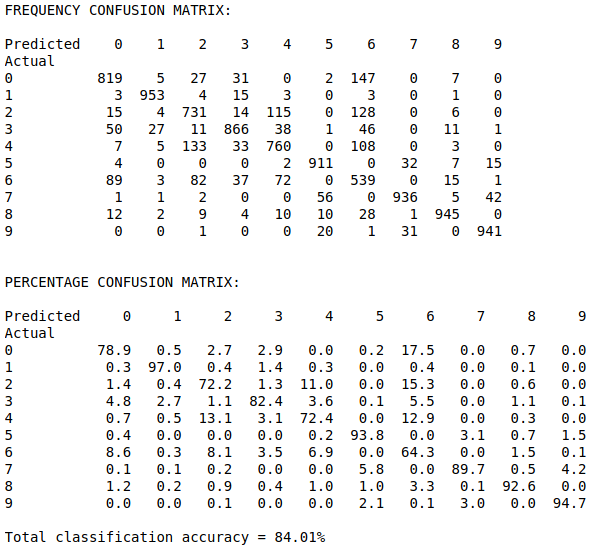
\includegraphics[width=0.7\textwidth]{images/q21.png}
        \end{center}
      \end{answerbox}
  


   \end{subquestion}
   %
   % ==============================
   %
   %==============================
   % Q2.2
   \begin{subquestion}{(3 points)
       Carry out a classification experiment with
       \href{https://scikit-learn.org/0.19/modules/generated/sklearn.svm.SVC.html}{SVM classifiers}, and report the
       mean accuracy and confusion matrix (in numbers) for the test
       set.
     } \label{Q2.2}


   

      \begin{answerbox}{30em}
        \begin{center}
        \textbf{\underline{Confusion matrices to show the classification accuracy of our trained}}\\
        \textbf{\underline{SVM model on the test set}}
        \vspace{0.3cm}\\
         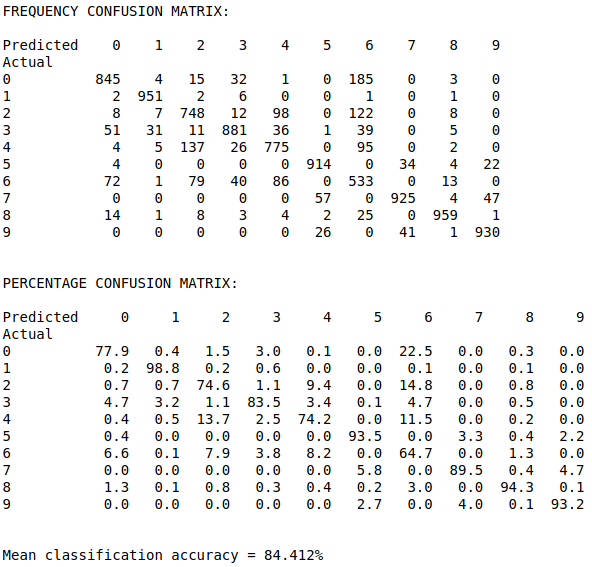
\includegraphics[width=0.7\textwidth]{images/q22.png}
        \end{center}
      \end{answerbox}
  


   \end{subquestion}
   %
   % ==============================
   %
   %==============================
   % Q2.3
   \begin{subquestion}{(6 points)
       We now want to visualise the decision regions for the logistic
       regression classifier we trained in \refQ{Q2.1}.
     } \label{Q2.3}


   

      \begin{answerbox}{35em}
        \begin{center}
         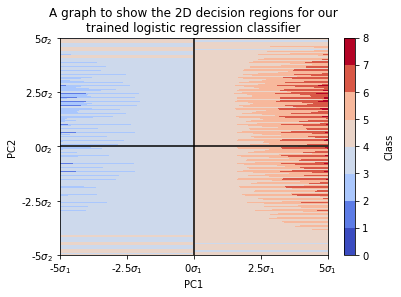
\includegraphics[width=0.7\textwidth]{images/q23.png}
        \end{center}
        \textbf{\footnotesize{\underline{Analysis of our results}}}\\
\\
        \scriptsize{
        I found the class distribution in this figure to be very surprising for these decision regions, especially given we have balanced classes in the training dataset. We can see there is no region for class 9 and that the regions for class 0, class 1, and class 7 are very small. We can deduce this is due to the fact that PCA can pick directions that make it hard to seperate classes, this is because PCA is unsupervised. Thereby there is a very good possibility this dimensionality reduction made the resulting transformed data not linearly seperable. This can be very problematic when using a linear model for classification like we are here (logistic regression model).\\
\\
        A solution to such a problem would be through either using LDA (Linear Discriminant Analysis) for dimensionality reduction instead of PCA, or choosing a classifier that is not linear (such as an SVM with an RBF kernel). I believe using LDA for dimensionality reduction would be the best solution in this context as in contrast to PCA this is a supervised technique and thereby reduces dimensions in order to maximize class seperability and thus we would not need to change our classifier. 
        }
      \end{answerbox}
  


   \end{subquestion}
   %
   % ==============================
   %
   %==============================
   % Q2.4
   \begin{subquestion}{(4 points)
       Using the same method as the one above, plot the decision regions for
       the SVM classifier you trained in \refQ{Q2.2}.
       Comparing the result with that you obtained in \refQ{Q2.3}, discuss your
       findings briefly.
     } \label{Q2.4}
   

      \begin{answerbox}{35em}
        \begin{center}
         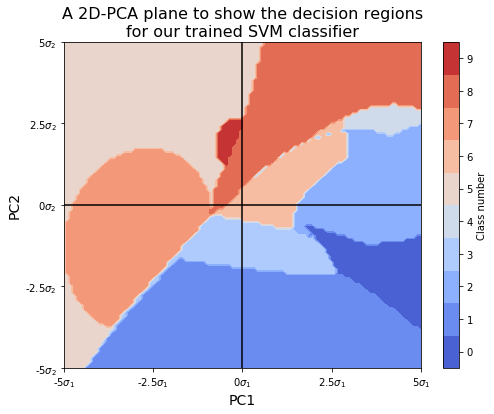
\includegraphics[width=0.7\textwidth]{images/q24.png}
        \end{center}
        \textbf{\footnotesize{\underline{Analysis of our results}}}\\
\\
        \scriptsize{
        These regions are far better than the ones we found in Q2.3 this is evident by the far more even class distribution. What is particularly exciting is how similar the layout of these decision regions are in comparison to the distribution of classes for our normalized training dataset once projected onto the 2D-PCA plane (that we found in Q1.8).\\
\\
        These decision regions have a very similar structure as the ones found in Q2.3, however, we can see they are far more well distributed as illustrated by the much more consistent size of regions, and inclusion of all the classes. We can deduce this difference is due to the fact that our data was made not linearly seperable by the PCA dimensionality reduction (as discussed in Q2.3), thus we can expect a SVM model with a nonlinear kernel (RBF) to seperate the data (and thus classify) far more effectively than a linear one such as our logistic regression model.
        }
      \end{answerbox}
  


   \end{subquestion}
   %
   % ==============================
   %

   %==============================
   % Q2.5
   \begin{subquestion}{(6 points)
       We used default parameters for the SVM in \refQ{Q2.2}.
       We now want to tune the parameters by using cross-validation.
       To reduce the time for experiments, you pick up the first 1000
       training samples from each class to create \texttt{Xsmall}, so that \texttt{Xsmall}
       contains 10,000 samples in total. Accordingly, you create
       labels, \texttt{Ysmall}.
     } \label{Q2.5}


   

      \begin{answerbox}{30em}
        \begin{center}
        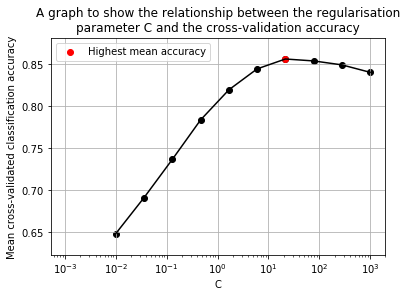
\includegraphics[width=0.6\textwidth]{images/q25.png}
        \end{center}
        \textbf{\underline{Optimal accuracy achieved and it's respective value of C:}} \\
        \\
        \footnotesize{$Accuracy \approx 85.65 \%$  where  $C = 10^{\frac{4}{3}}$}
      \end{answerbox}
  


   \end{subquestion}
   %
   % ==============================
   %
   %==============================
   % Q2.6
   \begin{subquestion}{(3 points)
       Train the SVM classifier on the whole training set by using the
       optimal value of $C$ you found in \refQ{Q2.5}. 
     } \label{Q2.6}


       

      \begin{answerbox}{10em}
        \textbf{\underline{Classification accuracy of our trained SVM model using the optimal}} \\
        \textbf{\underline{value of $\mathbf{C}$ found ($\mathbf{10^{\frac{4}{3}}}$)}}\\
        \\
        \footnotesize{
        Training accuracy $\approx 90.842\%$\\
        Testing accuracy $\approx 87.65\%$
        }
      \end{answerbox}
  


   \end{subquestion}
   %
   % ==============================
   %
%
%

\end{question}
%%%%%%%%%%%%%%%%%%%%%%%%%%%%%%%%%%%%%%%%%%%%%%%%%%%%%%%%%%%%%%%%%%%%%%%%%%%%%%
%============================================================================%
%%%%%%%%%%%%%%%%%%%%%%%%%%%%%%%%%%%%%%%%%%%%%%%%%%%%%%%%%%%%%%%%%%%%%%%%%%%%%%
\clearpage
%
% Question 3
%

\begin{question}{(20 total points) Clustering and Gaussian Mixture Models}  


  \questiontext{In this question we will explore K-means clustering,
    hierarchical clustering, and GMMs.
  }
  


  \medskip
   %==============================
   % Q3.1
   \begin{subquestion}{(3 points)
       Apply k-means clustering on {\tt Xtrn} for $k = 22$, where we use
       \href{https://scikit-learn.org/0.19/modules/generated/sklearn.cluster.KMeans.html}{sklearn.cluster.KMeans}
       with the parameters {\tt n\_clusters=22} and {\tt random\_state=1}.
       Report the sum of squared distances of samples to their closest
       cluster centre, and the number of samples for each cluster.
     } \label{Q3.1}
   

      \begin{answerbox}{35em}
        \textbf{\underline{Metrics for our trained k-means clustering model}}
        \vspace{0.3cm}\\
         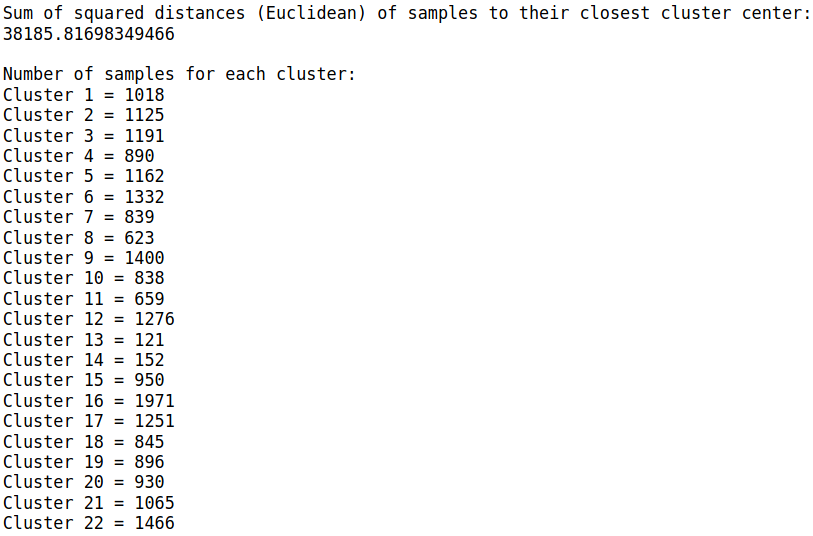
\includegraphics[width=1\textwidth]{images/q31.png}
      \end{answerbox}
  


   \end{subquestion}
   %
   % ==============================
   %
   %==============================
   % Q3.2
   \begin{subquestion}{(3 points)
       Using the training set only,
       calculate the mean vector for each language, and plot the mean
       vectors of all the 22 languages on a 2D-PCA plane, where you
       apply PCA on the set of 22 mean vectors without applying
       standardisation.  
       On the same figure, plot the cluster centres obtained in \refQ{Q3.1}.
     } \label{Q3.2}

   

      \begin{answerbox}{35em}
        \begin{center}
         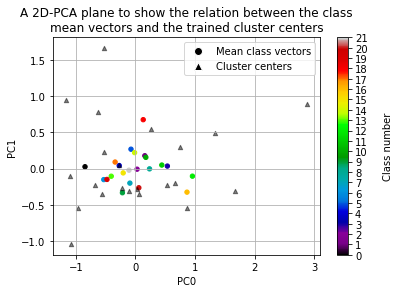
\includegraphics[width=0.63\textwidth]{images/q32.png}
        \end{center}
        \footnotesize{\textbf{\underline{Analysis of our results}}}\\
\\
        \scriptsize{
        We can see that most of the mean class vectors and clusters lie in the same general region of the plot with a few clusters more sparsely decorated. We can imagine these sparse clusters account for outliers in our data given that all the mean classes are in the same general region. \\
\\
        There is a cluster directly on top of class 4 which exemplifies the accuracy of this clustering. Although we cannot assume this cluster center was composed using purely data in this class alone,  we can imagine this class must have quite consistent data samples (low variance) throughout the dataset meaning small distances between samples and ultimately a very accurate cluster center.\\
\\
        What I found particularly interesting is the closely congregated collection of cluster centers where $-0.5 \leq PC2 \leq 0$, these lie just below the majority of the mean class vectors. I believe this is due to the fact that unlike the cluster centers the mean class vectors have been skewed by outliers. This is evident given the large amount of cluster centers with $PC2 \geq 0.5$. This is important to note, as means can be a misleading metric. This is due to the fact that they can be skewed greatly by outliers and they have no way of showing us the range of our data.
        }
      \end{answerbox}
  


   \end{subquestion}
   %
   % ==============================
   %
   %==============================
   % Q3.3
   \begin{subquestion}{(3 points)
       We now apply hierarchical clustering on the training data set
       to see if there are any structures in the spoken languages.
     } \label{Q3.3}


     

      \begin{answerbox}{35em}
        \begin{center}
        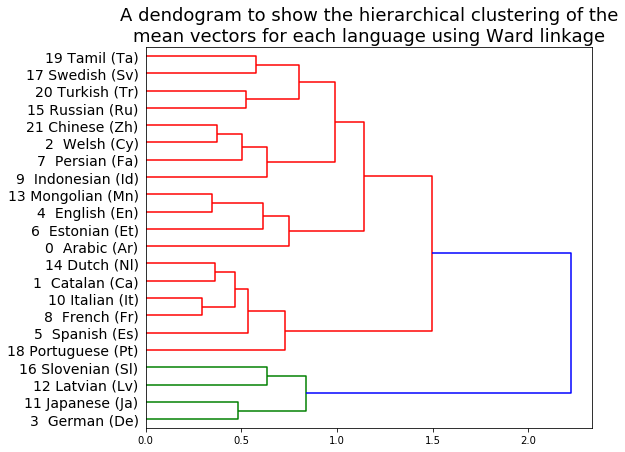
\includegraphics[width=0.68\textwidth]{images/q33.png}
        \end{center}
        \footnotesize{\textbf{\underline{Analysis of our results}}}\\
\\
        \scriptsize{
        This dendogram is very useful as it visually illustrates how each cluster from our dataset is composed and thus ultimately gives significant insight into the hierarchy of similarities between the classes in our data. This visualization makes it easy for us to determine the optimal number of clusters to fit to our data (ideally we want a cluster for each class to enable easy classification).\\
\\
        This clustering is not calculated by measuring the distance directly, but Ward linkage rather analyzes the variance of clusters and minimizes the total within-cluster variance of new cluster merges.\\
        \\
        From this dendogram, we can see that Italian and French have the most similar mean vectors given they have the smallest clustering distance and thereby are the most "similar" languages. In contrast we can see that Arabic has the most dissimilar mean vector from all other languages given it has the largest clustering distance and thereby is the most "unique" language.\\
\\
        If we had to choose an optimal number of clusters I believe a cut where distance $\approx 0.85$ (resulting in 5 clusters) would be most optimal due to the large merge clustering distance found after this cut, and also due to the fact we have lots of classes (22) meaning we would prefer more clusters to represent more detail in our data.
        }
      \end{answerbox}
  


   \end{subquestion}
   %
   % ==============================
   %
   %==============================
   % Q3.4
   \begin{subquestion}{(5 points)
       We here extend the hierarchical clustering done in \refQ{Q3.3} by
       using multiple samples from each language.
     } \label{Q3.4}


   

      \begin{answerbox}{50em}
        \begin{center}
        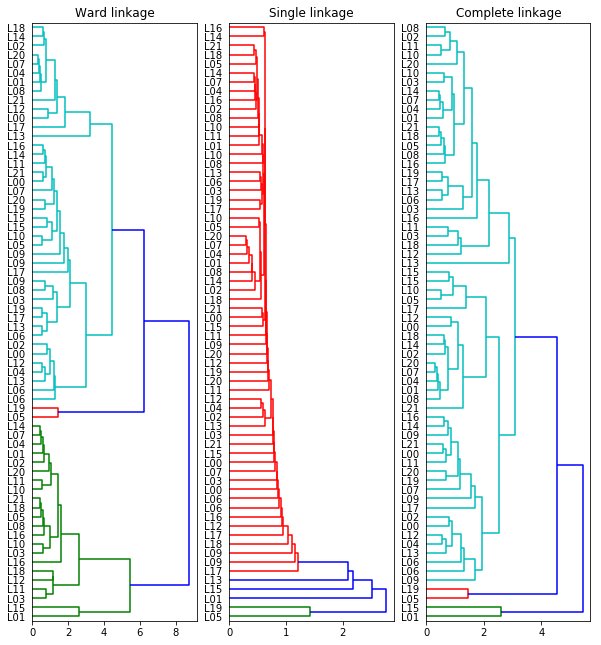
\includegraphics[width=0.7\textwidth]{images/q34.png}
        \end{center}
        \scriptsize{
        \emph{**The labels on all of these dendograms refer to the language that the given cluster center point came from.}\\
\\
\\
        \textbf{\footnotesize{\underline{Analysis of our results}}}\\
\\
        These dendograms are very useful as they make it easier for us to compare the results of varying linkage methods for hierarchical clustering on our data. This ultimately allows us to choose the method that produces the optimal results based on the classes in our data.\\
\\
        We can see that in all of these dendograms there is an isolated cluster for language 19 and 5. This suggests that this cluster is the most dissimimilar to all others among all different linkage criterion.\\
\\
        I believe single linkage is the least useful criterion in this context because of it's disproportionally large red cluster. The distances between all of the language cluster centers in this red section are on average very small (as illustrated by the scale on the x-axis) which make it far less useful as it does not seperate the different classes in a meaningful way.\\
\\
        I believe Ward linkage is the most useful as it has the largest overall distance between language cluster centers this is evident by looking at the scale of the x-axis in comparison to single and complete linkage. This larger distance ultimately impies higher variance in the data based on this criterion and thus is far more useful for classification.
        } 
      \end{answerbox}
  


   \end{subquestion}
   %
   % ==============================
   %
   %==============================
   % Q3.5
   \begin{subquestion}{(6 points)
       We now consider Gaussian mixture model (GMM), whose
       probability distribution function (pdf) is given as
       a linear combination of Gaussian or normal distributions, i.e.,
     } \label{Q3.5}




      \begin{answerbox}{30em}
        \scriptsize{
        \begin{center}
        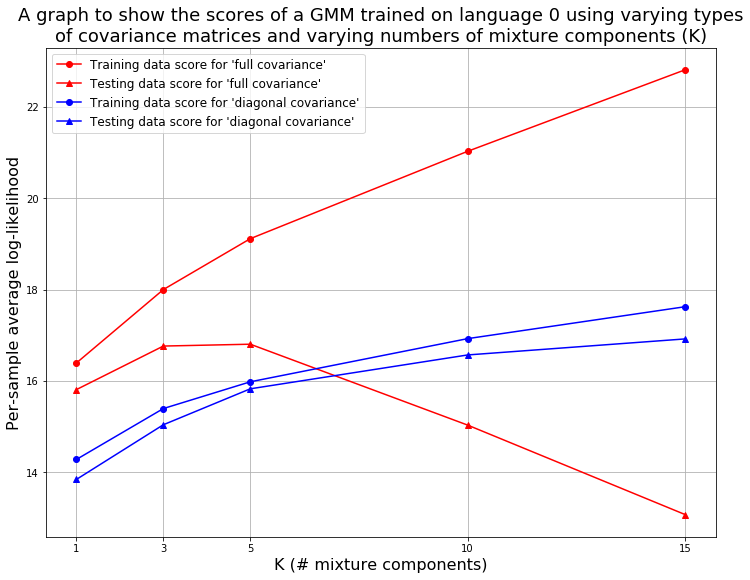
\includegraphics[width=0.6\textwidth]{images/q35.png}
        \end{center}
        \begin{center}
        \textbf{Table to show the average per-sample log-likelihood scores} \\
        \textbf{for varying parameters of a GMM} \\
        \vspace{0.3cm}
        \begin{tabular}{ |c|c|c|c|c|c|c| } \hline
        \textbf{Language 0 data} & \textbf{$\mathbf{\Sigma}$ type} & \textbf{K = 1} & \textbf{K = 3} & \textbf{K = 5} & \textbf{K = 10} & \textbf{K = 15} \\ \hline
        Training & Diagonal & 14.28 & 15.399 & 16.014 & 16.895 & 17.653 \\
        Testing & Diagonal & 13.843 & 15.041 & 15.882 & 16.375 & 19.942 \\
        Training & Full & 16.394 & 18 & 19.129 & 21.018 & 22.889 \\
        Testing & Full & 15.811 & 16.895 & 16.704 & 15.19 & 10.787 \\ \hline
        \end{tabular}
        \end{center}
        \textbf{\footnotesize{\underline{Analysis of our results}}}\\
\\
        The log-likelihood of a mixture model ultimately represents the probability of observing our data as a function of the model's parameters. Given this we know that the higher the per-sample average log-likelihood the better the accuracy of the model.\\
\\
        The only difference between these 2 models is the type of covariance matrix used. A full covariance matrix assumes data dependence and a diagonal covariance matrix assumes data independence. Thereby this graph is perfect for identifying if there are any relationships between variables in the data and choosing the optimal model for a given value of K.\\
\\ 
        As shown by the figure above we can see that the GMM model that uses the full covariance matrix has the best training accuracy by far, however, we can see this accuracy drops dramatically from $K > 3$ for the training data. We can attribute this to the fact that our model was overfit to our training data. This overfitting makes perfect sense due to the assumption of variable dependence. This assumed variable dependence ultimately makes our model far more susceptible for capturing false relationships between variables in the training dataset.\\
\\
        In contrast, the GMM model that uses the diagonal covariance matrix has a worse overall training accuracy, however, unlike for the full covariance model the testing accuracy does not drop as we increase K but rather stays consistent with it's respective training accuracy.
\\
\\
        In conclusion, we can deduce that for this dataset the number of mixture components (K) is inversely proportional to the dependence between variables in the dataset. Such that for $K \geq 8$ our GMM scores better when assuming data is dependent and visa-versa for when assuming data is independent.
        }
      \end{answerbox}
  


   \end{subquestion}
   %
   %==============================

   % ==============================
   
\end{question}
\end{document}
